\chapter{Current Limitations of Language Models}
\label{chapter:limitations}

\section{The Softmax Bottleneck}
\label{section:limitations:softmax_bottleneck}

The majority of parametric LMs use a Softmax function operating on the context $ c $ , and a word embedding $ e_w $ to define the conditional distribution $ P_\theta(w|c) $, where $ w $ stands for a word, and $ \theta $ are the parameters of the model. More specifically, the model distribution is usually written as:

\begin{displaymath}
    P_\theta(w | c) = \frac{h^Te_w}{\sum_{e_{w'}} h^Te_{w'}}
\end{displaymath}

Where $ h $ is a function of $ c $ and it is commonly obtained using a Recurrent Neural Network, and $ e_w $ is the embedding for word $ w $. Additionally, $ h \in R^D $ and $ e_w \in R^D $ and both \emph{h} and $ e_w $ depend on $ \theta $. Finally, we refer to the dot product $ h^Te_w $ as a \emph{logit}.

Even though, one might argue that natural languages contain an infinite amount of contexts, let's take a look at the finite case first. We can assume that a natural language consists of \emph{N} contexts and \emph{M} words. Consequently, we can describe Language Modelling as a matrix factorization problem. Consider the following matrices:

\begin{displaymath}
    \begin{matrix}
        H_\theta &= \begin{bmatrix}
               h^T_{c_1} \\
               h^T_{c_2} \\
               \vdots \\
               h^T_{c_N}
              \end{bmatrix}
        &     
        E_\theta &= \begin{bmatrix}
           e^T_{w_1} \\
           e^T_{w_2} \\
           \vdots \\
           e^T_{w_M}
          \end{bmatrix}
    \end{matrix} \\
\end{displaymath}
\begin{displaymath}
    \begin{matrix}
    A &= \begin{bmatrix}
       \log P(w_1 | c_1) & \log P(w_2 | c_1) & \hdots & \log P(w_M | c_1)  \\
       \log P(w_1 | c_2) & \log P(w_2 | c_2) & \hdots & \log P(w_M | c_2) \\
       \vdots & \vdots & \ddots & \vdots \\
       \log P(w_1 | c_N) & \log P(w_1 | c_N) & \hdots & \log P(w_M | c_N)
      \end{bmatrix}
    \end{matrix}
\end{displaymath}

Where $ H_\theta \in R^{N \times D} $ is a matrix containing the hidden states for every context as row vectors. $ E_\theta \in R^{M \times D}$ is a matrix containing word embeddings for every word as row vectors. $ A $ is a matrix containing the true log probabilities of every word, given every context. Then, language modelling can be described as:

\begin{displaymath}
    H_\theta E^T_\theta = \hat A
\end{displaymath}

Where, $ \hat A $ is:

\begin{displaymath}
    \begin{matrix}
    \hat A &= \begin{bmatrix}
       \log P_\theta(w_1 | c_1) & \log P_\theta(w_2 | c_1) & \hdots & \log P_\theta(w_M | c_1)  \\
       \log P_\theta(w_1 | c_2) & \log P_\theta(w_2 | c_2) & \hdots & \log P_\theta(w_M | c_2) \\
       \vdots & \vdots & \ddots & \vdots \\
       \log P_\theta(w_1 | c_N) & \log P_\theta(w_1 | c_N) & \hdots & \log P_\theta(w_M | c_N)
      \end{bmatrix}
    \end{matrix}
\end{displaymath}

and we want it to be as close as possible to the true $ A $. Now we can ask the following question:

\begin{center}
    \emph{"What is the expressiveness of this language model?"}
\end{center}

We can then proceed to answer this question from a matrix factorization point of view. Essentially, we want to learn matrices $ H_\theta $ and $ E_\theta $ such that we will be able to factorize the true distribution $ A $. However, in order for a valid factorization to exist the rank of $ H_\theta E^T_\theta $ has to be at least as large as the rank of $ A $, i.e. $ rank(H_\theta E^T_\theta ) >= rank(A) $. As $ H_\theta \in R^{N \times D} $ and $ E_\theta \in R^{M \times D} $, $ rank(H_\theta E^T_\theta ) $ is bounded by $ D $. Therefore, this is a limitation that comes from the final \emph{Softmax layer}. It simply means, that no matter how efficient we are in embedding all contexts into a matrix $ H_\theta $, we will not be able to retrieve the true language distribution $ A $, unless $ D >= rank(A) $.

To realize why this is indeed a bottleneck, and a problem in language modelling, we should first consider the typical dimensionalities that are used for the hidden state and the word embeddings. Usually, $ D $ is in the low hundreds, while the rank of the true distribution $ A $ can theoretically be up to $ M $ which is usually at least as large as $ 10^4 $. Right off the bat, we have a mismatch of several orders of magnitudes. One might say that an easy fix is to simply increase $ D $ and have a $ M \times M $ \emph{Softmax} in the final layer. However, this will drastically increase the amount of trainable parameters, resulting in slower training and harder optimization. Even though, wider and larger neural networks are theoretically more expressive, in practice they are a lot more difficult to train.

As using a larger $ D $ is not a straightforward solution to the problem it means that typical language models are \emph{Low Rank Language Models}. This would only cause problems if the true distribution $ A $ is indeed of a high rank. It is very hard to prove (if possible) that natural languages are of high rank. However, intuitively speaking, if the true distribution of a natural language was indeed to be of a low rank, it would mean that all semantic meanings can be created by combining a small number of meanings. Which seems very odd and no linguist has ever managed to find such a small subset of bases, which can fully describe a language. Therefore, \citet{yang2017breaking} speculate that a high rank language model is needed to capture the true distribution.

\section{Single Transformation}
\label{section:limitations:single_transformation}

Another limitation of classical language models is the output projection layer. Taking the matrix-vector product between the embedding matrix (nowadays weights between the output projection and the embedding matrix are usually tied) and the hidden state, further exponentiating and normalizing the result to get a probability distribution, essentially results in a transformation that behaves as a single mode Gaussian around the hidden state. This means that the majority of the probability mass is concentrated on one very small continuous subspace of the embedding space. This subspace usually corresponds to the surroundings of the word embedding that is mostly associated with the given context throughout training. Take the following sentence as an example:

\begin{center}
    \emph{“I want to buy…”}
\end{center}

It is easy to see that multiple words are likely to come after this particular context even though they might be associated with different contexts on average. This is a very common scenario in natural languages where the distribution over the vocabulary is considered to be a \emph{fat tail} distribution. For example take the words \emph{car} and \emph{computer}. By training a Language Model and plotting the embeddings, it is possible to visualize that the neighbors of \emph{car} in the embedding space are \emph{truck, auto, bus, vehicle} etc. and the neighbors of \emph{computer} are \emph{desktop, portable, electronic, laptop} etc. Refer to figures \ref{figure:car} and \ref{figure:computer}. This indicates that \emph{car} and \emph{computer} are in different neighborhoods of the embedding space.

\begin{figure}
\centering
\begin{subfigure}{.5\textwidth}
  \centering
  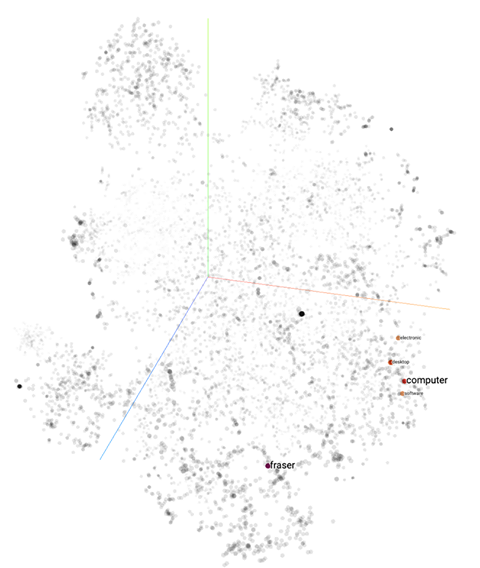
\includegraphics[width=\linewidth]{figures/computer_emb_neighbors.png}
%   \caption{A subfigure}
  \label{figure:car:neighborhood}
\end{subfigure}%
\begin{subfigure}{.5\textwidth}
  \centering
  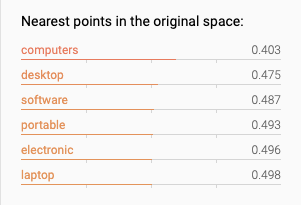
\includegraphics[width=\linewidth]{figures/computer_nearest_neighbors.png}
%   \caption{A subfigure}
  \label{figure:car:neighbor}
\end{subfigure}
\caption{Neighborhood of \emph{car} in the embedding space of AWD-LSTM.}
\label{figure:car}
\end{figure}

\begin{figure}
\centering
\begin{subfigure}{.5\textwidth}
  \centering
  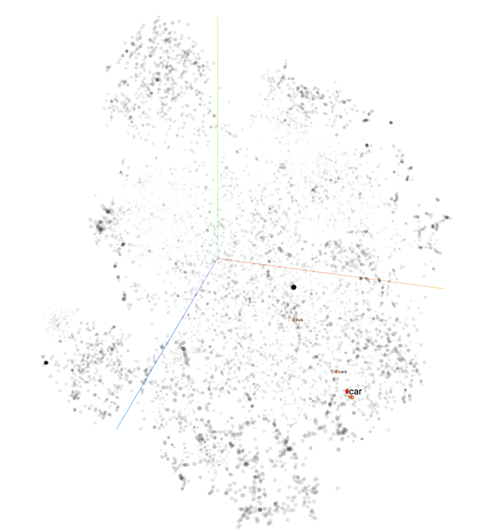
\includegraphics[width=\linewidth]{figures/car_emb_neighbor.png}
%   \caption{A subfigure}
  \label{figure:computer:neighborhood}
\end{subfigure}%
\begin{subfigure}{.5\textwidth}
  \centering
  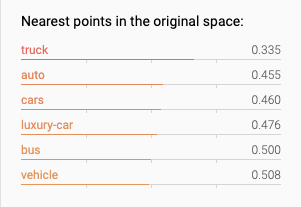
\includegraphics[width=\linewidth]{figures/car_nearest_neighbors.png}
%   \caption{A subfigure}
  \label{figure:computer:neighbor}
\end{subfigure}
\caption{Neighborhood of \emph{computer} in the embedding space of AWD-LSTM.}
\label{figure:computer}
\end{figure}

Now imagine every single word that can finish the previous sentence. Every one of those words is embedded into its own neighborhood where it is close to other words that share the same context on average. Therefore, a simple single mode Gaussian seems very limited for all those \emph{"fat tail"} situations in natural languages. Ideally, we would like something that can adapt based on the context, i.e. given a hidden state we can obtain different type of distributions. It is also possible that the success of MoS \citep{yang2017breaking} and DoC \citep{takase2018direct} papers, in addition to breaking the \emph{softmax bottleneck}, is due to the fact that they learn a dynamic mixture of Gaussians, which by definition is more expressive. Additionally, based on the amount of Gaussians in the mixture, those approaches are more or less capable of solving the previously mentioned issues.

To generalize, it seems unlikely that a single general distribution, conditioned on the hidden state, can capture all possible situations in Language Modelling. Therefore, it seems reasonable that based on the context, or the hidden state if you want, we would like to obtain custom distributions that specifically fit the need of the current context. But what if we can start with a "simple", single, general distribution and then based on the context, distort it into a more complex distribution if needed? That would alleviate the need to manually tune the amount of components in the mixture and can be seen as a generalization of MoS \citep{yang2017breaking} and DoC \citep{takase2018direct}.
